%%%%%%%%%%%%%%%%%%%%%%%%%%%%%%%%%%%%%%%%%%%%%%%%%%%%%%%%%%%%%%%%%%%%%%%%%%%
%
% Plantilla para un artículo en LaTeX en doble columna.
%
%%%%%%%%%%%%%%%%%%%%%%%%%%%%%%%%%%%%%%%%%%%%%%%%%%%%%%%%%%%%%%%%%%%%%%%%%%
% !TeX spellcheck = es_ANY
%\documentclass[11pt,twocolumn]{article} %doble columna
%\documentclass[11pt]{article}

\documentclass[conference]{IEEEtran}
\IEEEoverridecommandlockouts
% The preceding line is only needed to identify funding in the first footnote. If that is unneeded, please comment it out.

\usepackage{url}
\usepackage[utf8]{inputenc}
\usepackage[english]{babel}
\usepackage{fullpage}
\usepackage{graphicx}
\usepackage{array}

% Paquetes de la AMS:
\usepackage{amsmath, amsthm, amsfonts, amssymb}

% Atajos.
% Se pueden definir comandos nuevos para acortar cosas que se usan
% frecuentemente. Como ejemplo, aquí se definen la R y la Z dobles que
% suelen representar a los conjuntos de números reales y enteros.
%--------------------------------------------------------------------------

\def\RR{\mathbb{R}}
\def\ZZ{\mathbb{Z}}

% De la misma forma se pueden definir comandos con argumentos. Por
% ejemplo, aquí definimos un comando para escribir el valor absoluto
% de algo más fácilmente.
%--------------------------------------------------------------------------
\newcommand{\abs}[1]{\left\vert#1\right\vert}


%--------------------------------------------------------------------------
\title{Identification of rice genes which respond to saline stress from co-expression networks analysis}
\author{Camila Riccio Rengifo\\
  \small Pontificia Universidad Javeriana Cali\\
}

\begin{document}

\maketitle

\begin{abstract}
A gene co-expression network is an undirected graph , where each node corresponds to a gene, and a pair of nodes is connected if there is a significant co-expression relationship between them, that is, if they show similar expression patterns. These co-expression networks are of biological interest since the co-expressed genes are usually controlled by the same transcriptional regulatory pathway, functionally related or members of the same pathway or metabolic complex. Weighted gene co-expression network analysis (WGCNA)  is a method of data mining widely used to build co-expression networks, identify groups (modules) of highly correlated genes and relate these modules to external traits.

The aim of this work is to identify rice genes that respond to saline stress. The methodology is based on WGCNA with a new aproach in the modules detection, using  the hierarchical link clustering (HLC) technique that allows the recognition of overlapping communities, which may have more biological meaning given the overlapping regulatory domains of systems that generate coexpression \cite{gaiteri2014beyond}. Finally the LASSO method is used to select the most significant modules associated with rice phenotypical responses to salt stress. The genes differentially expressed within the selected modules are enriched with gene ontology annotations and their interaction networks are studied.
%\keywords{First keyword  \and Second keyword \and Another keyword.}
\end{abstract}


\section*{Introduction}
Introduction text

\section{Methodology}
\subsection{Data pre-processing} 
%-----------------------------
% RNA-seq data
%-----------------------------
RNA-seq data was accessed through GEO database \cite{GEOAcces90:online} (Accession number GSE98455), corresponding to $n=57845$ gene expression profiles of shoot tissues measured for both control and salt condition in $p=92$ accessions of the Rice Diversity Panel 1 (with two biological repetitions). \\

The RNA-seq data cannot be directly interpreted, therefore a normalization process has to be done to deal with the various biases that affect quantification results. The normalization tecnique used was DESeq2 \cite{love2014moderated}. From the normalized data, the two biological repetitions of each accession were averaged and genes exhibiting low variance (the ratio of upper quantile to lower quantile smaller than 1.5) or low expression (more than 80\% samples with values smaller than 10) were removed. At this point, control and salinity stress treatment data are separated into two matrices $C=[c_{ij}]_{n \times p}$ and $T=[t_{ij}]_{n \times p}$, respectively, where $c_{ij}$ and $t_{ij}$ represent normalized expression level of the gene $i$ in the accession $j$.

Changes in gene expression between control and stress conditions, are measured in terms of log ratios. Matrix $E=[e_{ij}]_{n \times p}$, known as the Log Fold Change matrix, is computed by setting $e_{ij}=\log_2 (t_{ij}/c_{ij})$. 

Genes with the ratio of upper quantile to lower quantile larger than $0.25$ were kept. This procedure aims to remove genes with low variance in the differential expression paterns. The final network contains $8928$ genes of the initial $57845$.


\subsection{Network construction}
The co-expression network is constructed based on WGCNA, as explained below.\\

The Log Fold Change matrix is used to construct the weighted co-expression network using the absolute value of the Pearson correlation as the similarity measure between genes. The matrix $S=[s_{ij}]_{n\times n}$ measures the level of concordance between gene expression profiles across experiments and is transformed into an adjacency matrix $A=[a_{ij}]_{n\times n}$ where $a_{ij} = (s_{ij})^\beta $ encodes the connection strength between each pair of genes. In other words, the elements of the adjacency matrix are the similarity values up to the power $\beta > 1$ so the degree distribution will fit a scale-free network. This kind of networks contain many nodes with very few connections and a small number of hubs with high connections. \\

In a strict scale-free network the logarithm of $P(k)$ (the probability of a node to have degree $k$) is approximately inversely proportional to the logarithm of $k$ (the degree of a node). So the parameter $\beta$ is chosen as the smallest value of $\beta$ such that the $R^2$ of the linear regression between $log_{10}(p(k))$ and $log_{10}(k)$ is close to $1$ (e.g. $R^2 > 0.85$). Figure~\ref{fig:beta} shows the degree distribution of the similarity matrix (left) and the degree distribution of the adjacency matrix (rigth) which is the degree distribution of a scale-free forced network with $R^2 = 0.8$ corresponding to $\beta = 3$.

%scale-free beta 1 y 3
\begin{figure}[h]
  \centering
    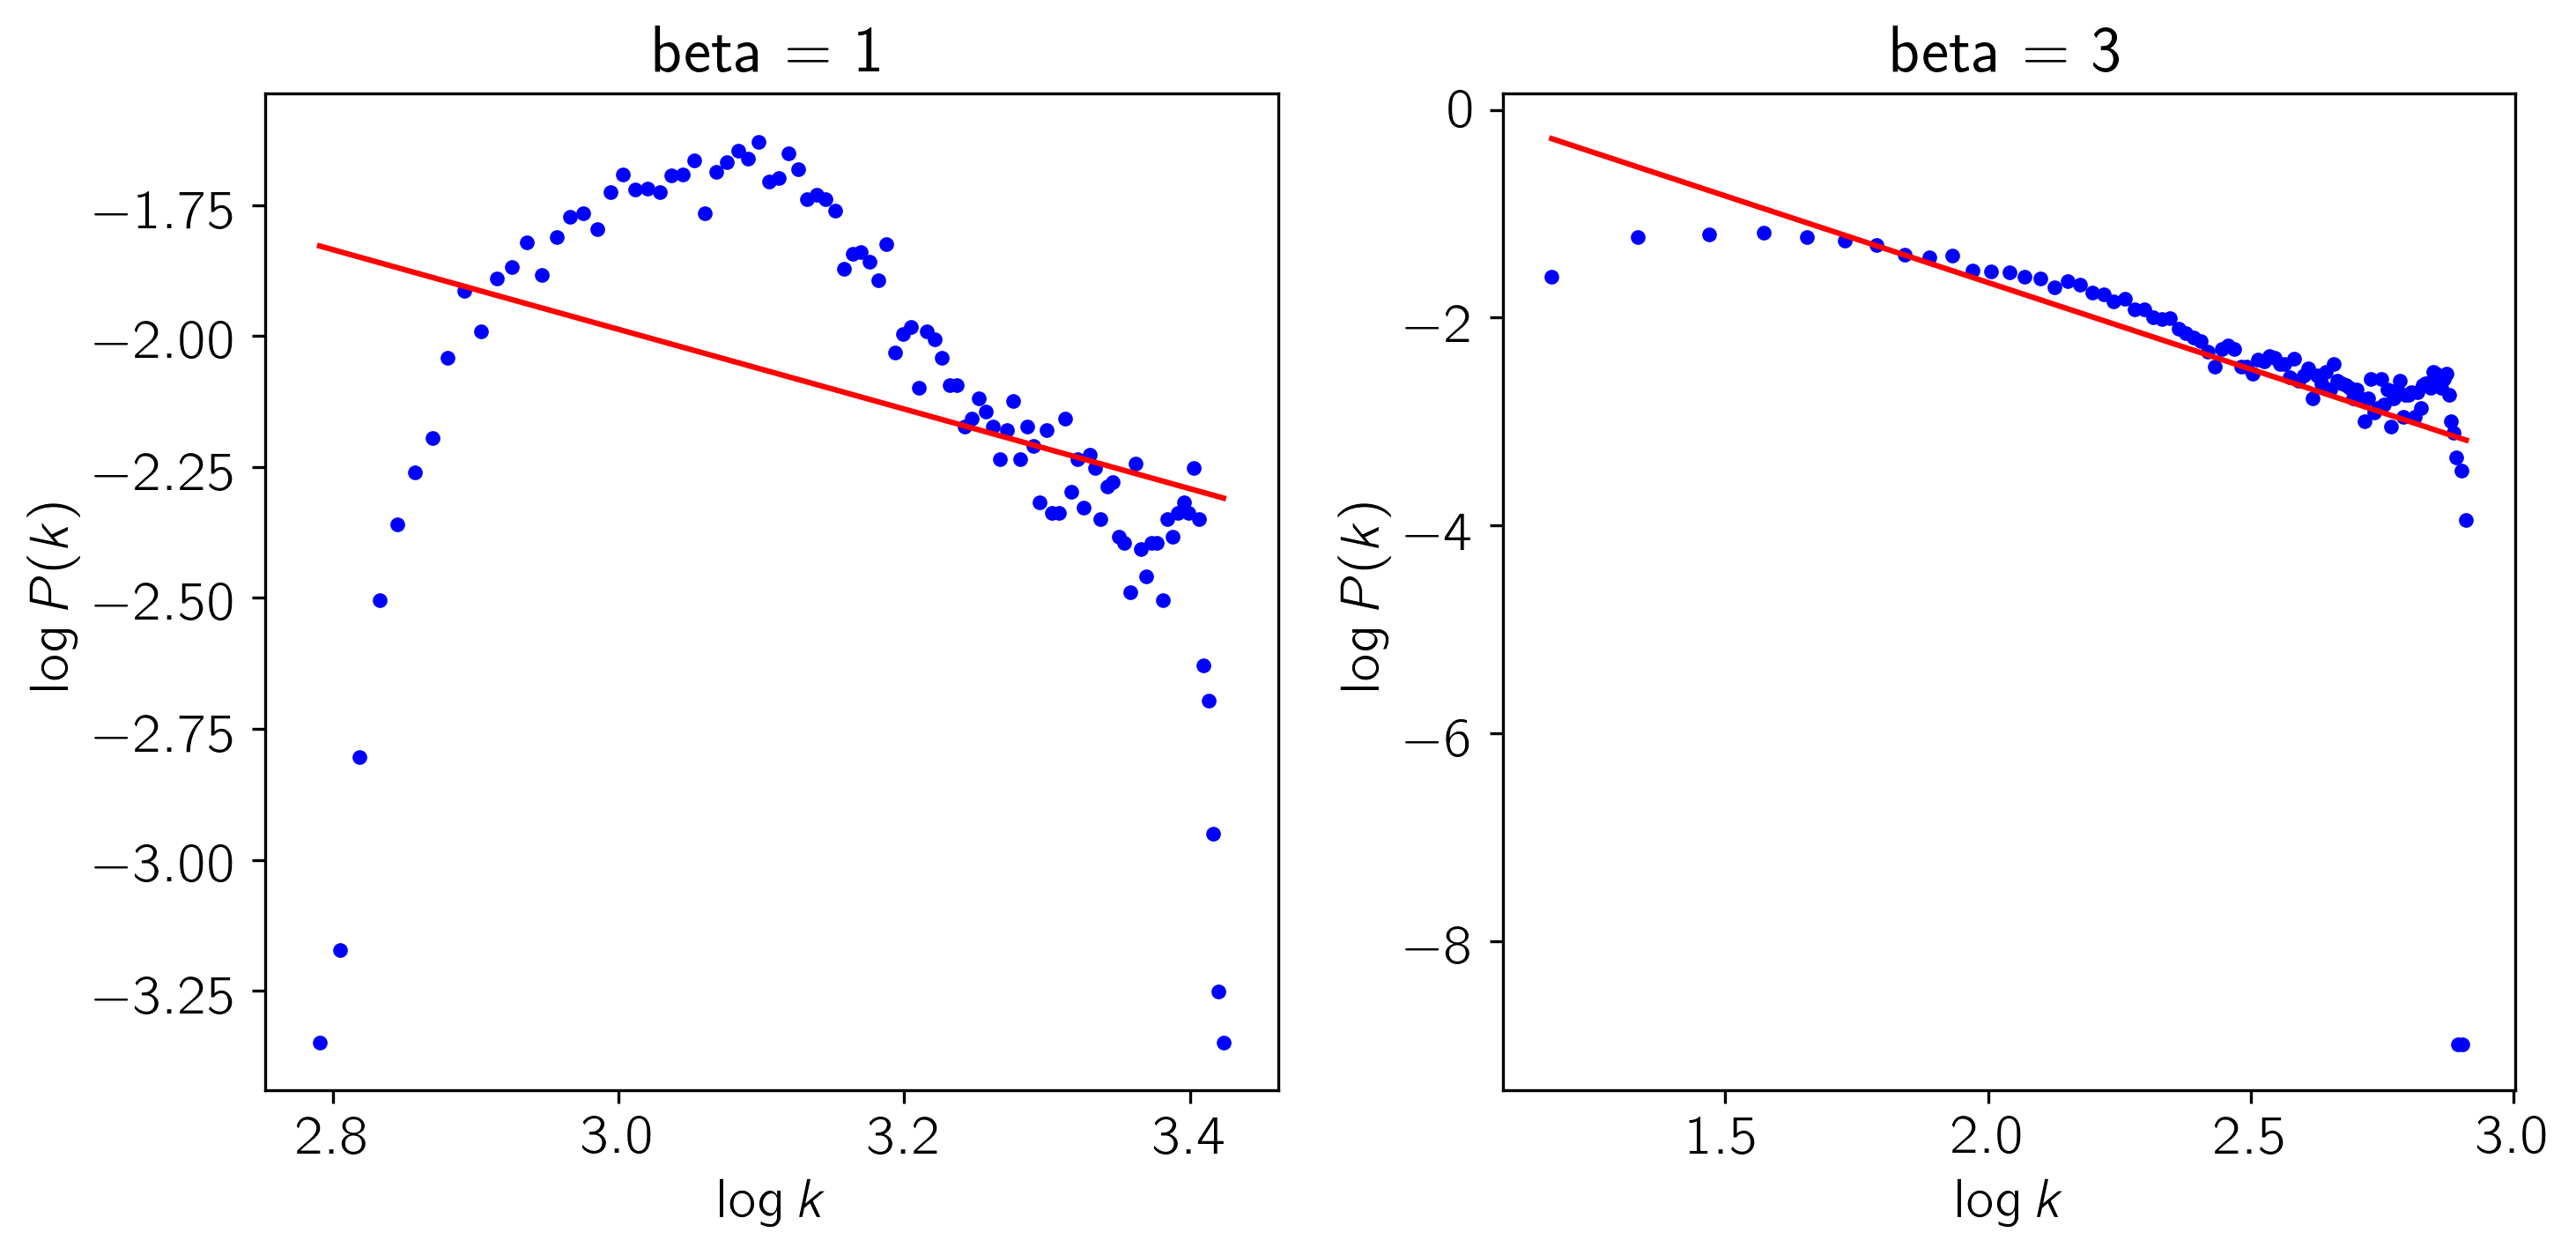
\includegraphics[clip,width=0.4\textwidth]{Figures/pick_beta.png}
  \caption{Degree distributions}
  \label{fig:beta}
\end{figure}

\subsection{Module detection}	
Once the network has been constructed, the next step is to study its structure and dynamics identifying communities also called modules. Membership in these modules may overlap in biological contexts, where modules may be related to specific molecular, cellular or tissue functions and the biological components (i.e. genes) are involved in multiple functions.\\

To identify these overlapping communities we make use of the Hierarchical Link Clustering (HLC) algorithm proposed in~\cite{ahn2010link}. HLC aproach reinvent communities as groups of links rather than nodes, each node inherits all memberships of its links and can thus belong to multiple, overlapping communities. The algorithm maps links to nodes and connects them if a pair of links shares a node. They compute the similarity between links using the Jaccard index for unweigthed networks and the tanimoto coefficient for weighted networks. With this similarity, they use single-linkage hierarchical clustering to build a dendrogram where each leaf is a link from the original network and branches represent link communities. Finally, the most relevant communities are established at the maximal partition density, a function  based on link density inside communities.\\

The current network represented by the adjacency matrix $A$, corresponds to a complete and weigthed network of $8,928$ genes (nodes) and $39,850,128$ edges. For computational reasons, this network was transformed into an unweighted one $\hat{A}$, keeping only the connections above the cutoff value of $0.2$. The resulting unweighted network has a total of $5,810$ nodes and $16,875,145$ edges. After applying the HLC algorithm, a total of $4,131$ genes were distributed in $5,143$ overlapping modules of $3$ or more genes. Figure~\ref{fig:overlap} shows a histogram of the overlapping percentage of these genes, measured as the proportion of modules to which each gene belongs.\\

%overlapping percentage
\begin{figure}[h]
  \centering
    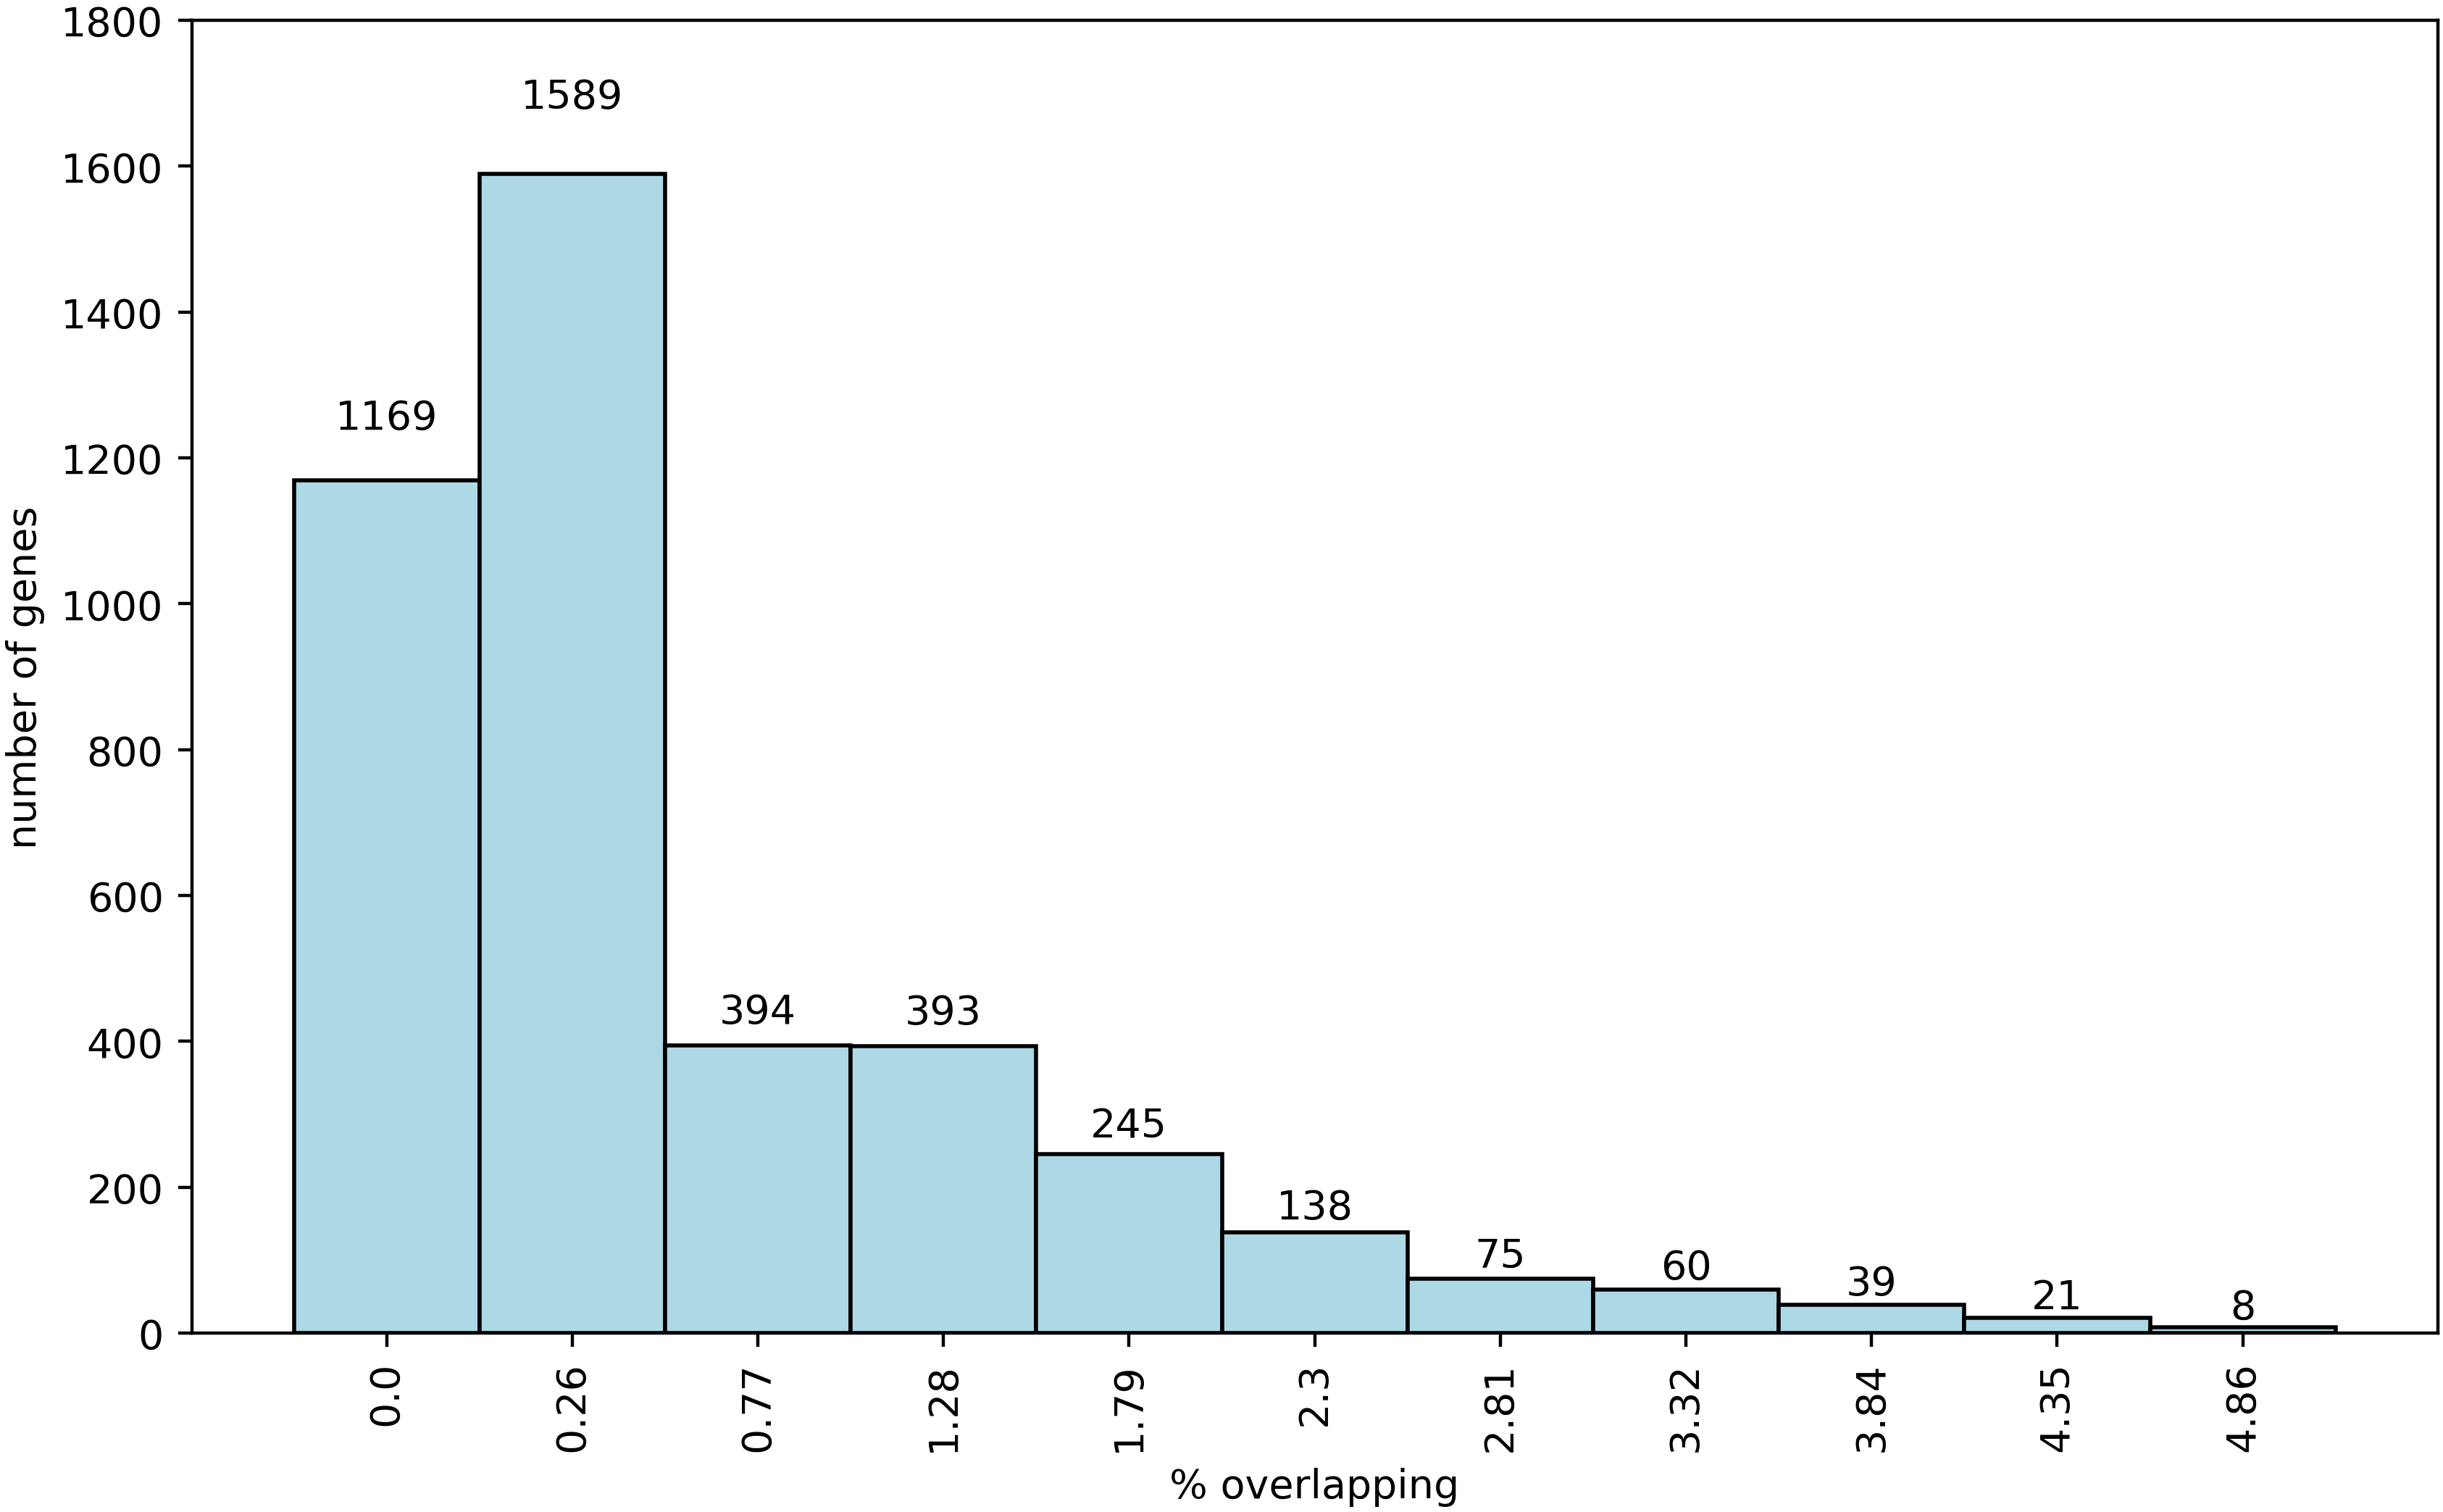
\includegraphics[clip,width=0.4\textwidth]{Figures/artificial_modules.png}
  \caption{Overlapping percentage}
  \label{fig:overlap}
\end{figure}

\subsection{Modules association to phenotypic traits}

Our approach to identify the most relevant gene groups (modules) in the response to salt stress, consists in relating the co-expression network with phenotypic data from the samples. We use 3 phenotypic traits: shoot $K^+$ content, root biomass and shoot biomass. These were measured for the 92 genotypes studied, under  control and salt stress conditions. These data can be found in the supplementary information of~\cite{campbell2017allelic}. As shown in Figure \ref{fig:pdata}, there are significant differences in the values of these phenotypic traits between both stress and control conditions. This supports the idea that these variables represent tolerance-associated traits in rice under salt stress.\\

% boxplots
\begin{figure}[h]
  \centering
    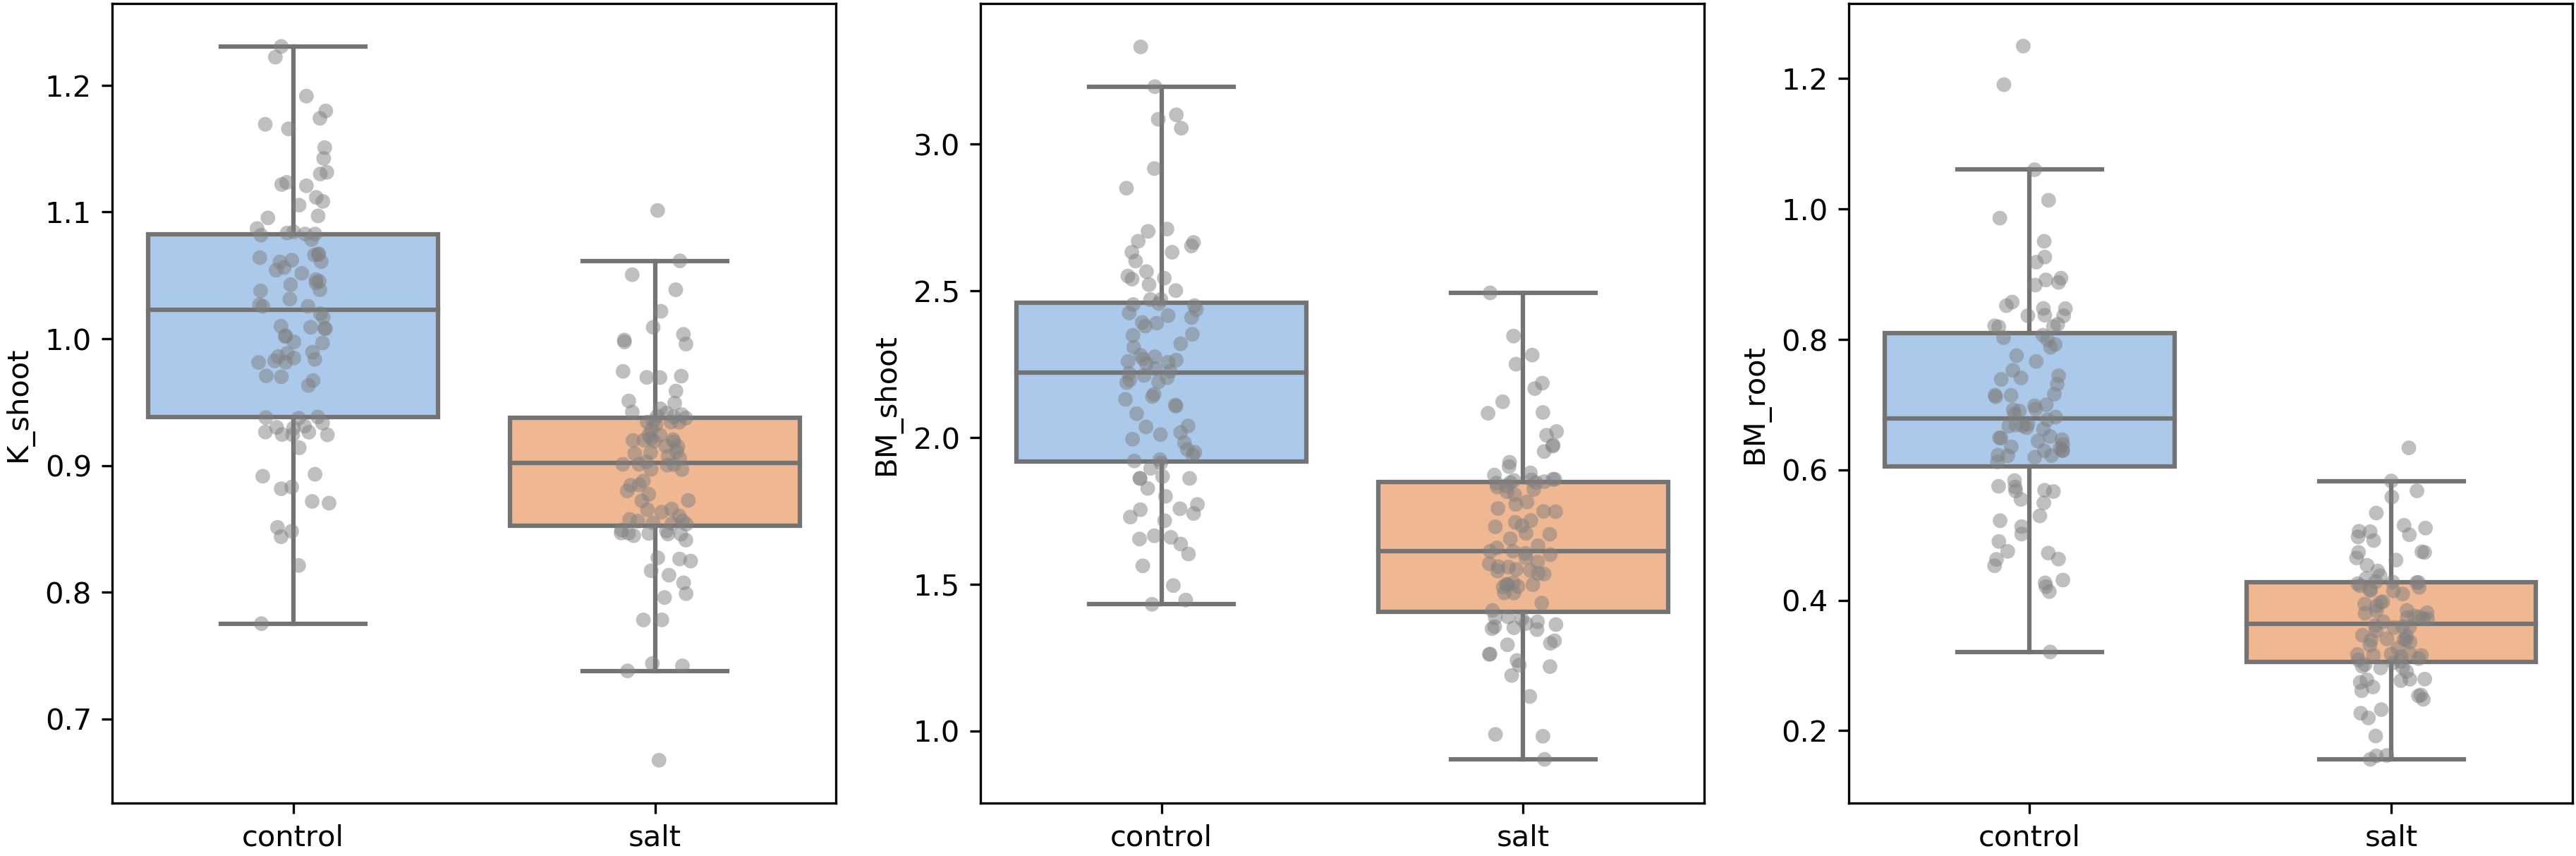
\includegraphics[clip,width=0.5\textwidth]{Figures/phenotypic_traits.png}
  \caption{Phenotipic traits distribution under control and salt stress}
  \label{fig:pdata}
\end{figure}

In order to relate the modules to the phenotypic traits, we represent each module with the first principal component of the Log Fold Change submatrix, corresponding to the genes of such module, which can be thought of as an average differential expression profile for each community. These profiles are then associated with each phenotypic trait using the LASSO variable selection method, allowing to identify a set of relevant modules related to the response to salinity conditions in rice plants. See Appendix A for a LASSO method description.\\

%Módulos seleccionados + cantidad de genes por módulo

\subsection{Genes enrichment}
% genes seleccionados con expresión diferencial según análisis DEA. 
% gene ontology de esos genes

\section{Results}
% redes de los genes anotados

\section{Discussion}


\bibliographystyle{acm}
\bibliography{mybibliography}

\newpage
\section*{Appendix}
\subsection{A: Variable selection with LASSO}
LASSO (Least Absolute Shrinkage Selector Operator) is a regularized linear regression technique, a method that combines a regression model with a procedure of contraction of some parameters towards zero and selection of variables, imposing a restriction or a penalty on the regression coefficients. Very usefull in problems where the number of variables (genes) $ n $ is much greater than the number of samples $ p $ ($ n \gg p $). Lasso solves the least squares problem with restriction on the $ L_1$-norm of the coefficient vector:

\begin{equation}
\min \left\lbrace\sum_{i=1}^{p}{\left( y_i-\sum_{j=1}^n{\beta_j x_{ij}}\right)^2} \right\rbrace , \textrm{sujeto a} \sum_{j=1}^n\abs{\beta_j}\leq s
\end{equation}

Or equivalently minimizing:
\begin{equation}
\sum_{i=1}^{p}{\left( y_i-\sum_{j=1}^n{\beta_j x_{ij}}\right)^2} + \lambda \sum_{j=1}^n\abs{\beta_j}
\end{equation}
being $ s $, $ \lambda \geq 0 $ the respective penalty parameters for complexity.\\

%LASSO produces parameter estimation and simultaneous variable selection for increasing values of $ \lambda $.

%if $ \lambda = 0 $ the estimator corresponds to the ordinary least squares estimator.

Since the $\lambda$ value determines the degree of penality, the accuracy of the model depends on its choice. Cross-validation is often used to select the regularization parameter, choosing the one that minimizes the mean-squered error. With that selected $\lambda$ value, the model is adjusted again, this time using all the observations.\\

In the module gene selection context, the outcome variable correspond to the phenotipic trait, whereas the predictors are the modules, detected by the hierarchical clustering, represented by the first principal component of the module. After running the Lasso regression will select the most significant modules associated with phenotyping data.  


\end{document}
